\documentclass{article}
\usepackage{graphicx}
\usepackage{amsmath,amsthm,amssymb}
\usepackage{mathtools}
\usepackage[font=small,labelfont=bf]{caption}
\usepackage{tikz}
\usetikzlibrary{calc, angles, quotes, shapes.geometric, decorations.pathreplacing, patterns}
\usepackage{tkz-euclide}
\usepackage{float}
\usepackage[margin=1in]{geometry}
\usepackage{gensymb}
\usepackage[normalem]{ulem}
\usepackage{fancyhdr}
\pagestyle{fancy}
\fancyhead[R]{Enoch Yu}
\pagenumbering{gobble}
\usepackage{hyperref}
\hypersetup{
    colorlinks=true,
    linkcolor=blue,
    filecolor=magenta,      
    urlcolor=cyan,
    pdftitle={Overleaf Example},
    pdfpagemode=FullScreen,
    }
\usepackage{enumitem}
\newtheorem{theorem}{Theorem}[section]
\newtheorem{lemma}[theorem]{Lemma}
\newtheorem*{lemma*}{Lemma}
\newtheorem{sublemma}{Lemma}[section]
\newtheorem{proposition}{Proposition}
\newtheorem{corollary}{Corollary}[theorem]
\newtheorem{example}{Example}[section]
\newtheorem*{example*}{Example}
\newenvironment{solution}{\begin{trivlist}\item[]{\bf Solution}}{\qed \end{trivlist}}
\newcommand{\verteq}{\rotatebox{90}{$\;\;=\;\;$}}
\newcommand*\circled[1]{\tikz[baseline=(char.base)]{
            \node[shape=circle,draw,inner sep=1pt] (char) {#1};}}
\newcommand{\triangled}[1]{\tikz[baseline=(char.base)]{
            \node[shape=regular polygon, regular polygon sides=3, draw, inner sep=0.2pt] (char) {#1};}}

\title{Problem Set 31}
\author{Enoch Yu}
\date{July 2025}

\begin{document}

\section*{2018 AMC 12A Problem 22}
The solutions to the equations $z^2=4+4\sqrt{15}i$ and $z^2=2+2\sqrt 3i,$ where $i=\sqrt{-1},$ form the vertices of a parallelogram in the complex plane. The area of this parallelogram can be written in the form $p\sqrt q-r\sqrt s,$ where $p,$ $q,$ $r,$ and $s$ are positive integers and neither $q$ nor $s$ is divisible by the square of any prime number. What is $p+q+r+s?$
\\\\
$\textbf{(A) } 20 \qquad  \textbf{(B) } 21 \qquad  \textbf{(C) } 22 \qquad  \textbf{(D) } 23 \qquad  \textbf{(E) } 24$
\begin{solution}
\\\\
\textbf{Key Words} Shoelace Formula
\\\\
\begin{minipage}[t]{0.5\textwidth}
Notice the following equalities.
\begin{align*}
    4 + 4\sqrt{15}i
    &= 4 + 2\sqrt{60}i \\
    &= \left( \sqrt{10} + \sqrt{6}i \right)^2
\end{align*}
In other words, the two roots for $z$ in the first equation are $\pm \sqrt{10} \pm \sqrt{6}i$.
\end{minipage}
\begin{minipage}[t]{0.5\textwidth}
Similarly,
\begin{align*}
    2 + 2\sqrt{3}i
    &= \left( \sqrt{3} + i \right)^2
\end{align*}
Thus, the two roots for $z$ in the first equation are $\pm \sqrt{3} \pm i$.
\end{minipage}
\\\\\\
Using the shoelace formula, the area of the parallelogram could be computed.
\begin{align*}
    \text{Area} &= \frac{1}{2}
    \begin{vmatrix}
        \sqrt{10} & -\sqrt{3} & -\sqrt{10} & \sqrt{3} & \sqrt{10} \\
        \sqrt{6} & -1 & -\sqrt{6} & 1 & \sqrt{6}
    \end{vmatrix} \\[0.5em]
    &= \frac{1}{2} \Big\{ \left( -\sqrt{10} + \sqrt{18} - \sqrt{10} + \sqrt{18} \right) - \left( -\sqrt{18} + \sqrt{10} - \sqrt{18} + \sqrt{10} \right) \Big\} \\[0.5em]
    &= 2\sqrt{18} - 2\sqrt{10} \\[0.5em]
    &= 6\sqrt{2} - 2\sqrt{10}
\end{align*}
Therefore, $6 + 2 + 2 + 10 = \boxed{\textbf{(A) } 20}$.
\end{solution}

\newpage
\section*{2018 AMC 12A Problem 23}
In $\triangle PAT,$ $\angle P=36^{\circ},$ $\angle A=56^{\circ},$ and $PA=10.$ Points $U$ and $G$ lie on sides $\overline{TP}$ and $\overline{TA},$ respectively, so that $PU=AG=1.$ Let $M$ and $N$ be the midpoints of segments $\overline{PA}$ and $\overline{UG},$ respectively. What is the degree measure of the acute angle formed by lines $MN$ and $PA?$
\\\\
$\textbf{(A) } 76 \qquad  \textbf{(B) } 77 \qquad  \textbf{(C) } 78 \qquad  \textbf{(D) } 79 \qquad  \textbf{(E) } 80$
\\\\
\textbf{Solution I.}
\\\\
\begin{minipage}[t]{0.5\textwidth}
First and foremost, draw the diagram.
\begin{center}
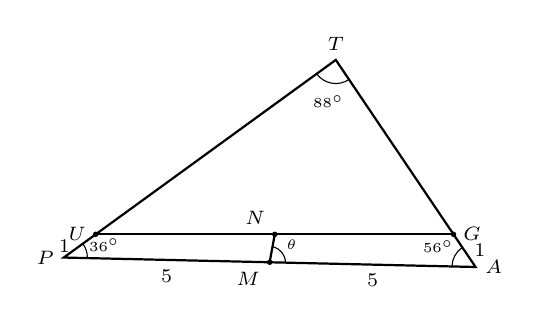
\begin{tikzpicture}[scale=0.5]
    \coordinate (A) at (11.6, 0.59);
    \coordinate (P) at (1.14, 0.83);
    \coordinate (T) at (8.05, 5.85);
    \coordinate (M) at (6.37, 0.71);
    \coordinate (N) at (6.5, 1.42);
    \coordinate (G) at (11.04, 1.42);
    \coordinate (U) at (1.95, 1.42);

    \coordinate (V1) at (0, 0);
    \coordinate (V2) at (12, 0);
    \coordinate (V3) at (1.7, 0);
    \coordinate (V4) at (10.79, 0);
    \coordinate (V5) at (6.25, 0);

    \draw[thick] (A) -- (P) -- (T) -- cycle;
    \draw[thick] (G) -- (U);
    \draw[thick] (M) -- (N);

    \foreach \n in {G, U, M, N}
        \node at (\n)[circle,fill,inner sep=0.7pt]{};
    
    \draw pic["\tiny $36^\circ$", draw=black, angle radius=0.3cm, angle eccentricity=1.8] {angle=A--P--T};
    \draw pic["\tiny $56^\circ$", draw=black, angle radius=0.3cm, angle eccentricity=1.8] {angle=T--A--P};
    \draw pic["\tiny $88^\circ$", draw=black, angle radius=0.3cm, angle eccentricity=1.8] {angle=P--T--A};
    \draw pic["\tiny $\theta$", draw=black, angle radius=0.2cm, angle eccentricity=1.8] {angle=A--M--N};
    
    \node[right] at (A) {\scriptsize $A$};
    \node[left] at (P) {\scriptsize $P$};
    \node[above] at (T) {\scriptsize $T$};
    \node[left] at (U) {\scriptsize $U$};
    \node[right] at (G) {\scriptsize $G$};
    \node[above left] at (N) {\scriptsize $N$};
    \node[below left] at (M) {\scriptsize $M$};
    \node[below] at ($(P)!0.5!(M)$) {\scriptsize $5$};
    \node[below] at ($(M)!0.5!(A)$) {\scriptsize $5$};
    \node[left] at ($(P)!0.5!(U)$) {\scriptsize $1$};
    \node[right] at ($(G)!0.5!(A)$) {\scriptsize $1$};
\end{tikzpicture}
\end{center}
\end{minipage}
\begin{minipage}[t]{0.5\textwidth}
In order to use the angles $36^\circ$ and $56^\circ$ and midpoints, the quadrilateral could be attached through rotation.
\begin{center}
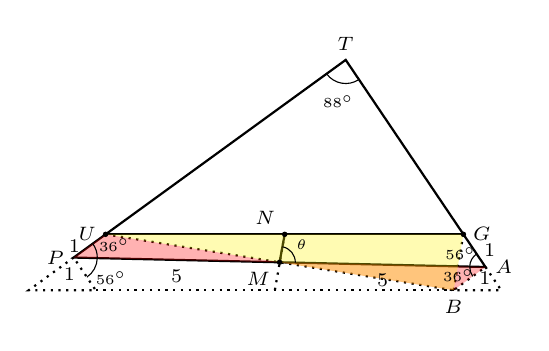
\begin{tikzpicture}[scale=0.5]
    \coordinate (A) at (11.6, 0.59);
    \coordinate (P) at (1.14, 0.83);
    \coordinate (T) at (8.05, 5.85);
    \coordinate (M) at (6.37, 0.71);
    \coordinate (N) at (6.5, 1.42);
    \coordinate (G) at (11.04, 1.42);
    \coordinate (U) at (1.95, 1.42);

    \coordinate (V1) at (0, 0);
    \coordinate (V2) at (12, 0);
    \coordinate (V3) at (1.7, 0);
    \coordinate (V4) at (10.79, 0);
    \coordinate (V5) at (6.25, 0);

    \draw[thick] (A) -- (P) -- (T) -- cycle;
    \draw[thick] (G) -- (U);
    \draw[thick] (M) -- (N);
    \draw[dotted, thick] (P) -- (V1) -- (V3) -- cycle;
    \draw[dotted, thick] (A) -- (V2) -- (V4) -- cycle;
    \draw[dotted, thick] (V3) -- (V4);
    \draw[dotted, thick] (U) -- (V4);
    \draw[dotted, thick] (G) -- (V4);
    \draw[dotted, thick] (N) -- (V5);

    \fill[red, opacity=0.3] (U) -- (P) -- (M);
    \fill[red, opacity=0.3] (A) -- (V4) -- (M);
    \fill[yellow, opacity=0.3] (U) -- (V4) -- (G);

    \foreach \n in {G, U, M, N}
        \node at (\n)[circle,fill,inner sep=0.7pt]{};
    
    \draw pic["\tiny $36^\circ$", draw=black, angle radius=0.3cm, angle eccentricity=1.8] {angle=A--P--T};
    \draw pic["\tiny $56^\circ$", draw=black, angle radius=0.2cm, angle eccentricity=1.8] {angle=T--A--P};
    \draw pic["\tiny $36^\circ$", draw=black, angle radius=0.2cm, angle eccentricity=1.8] {angle=M--A--V4};
    \draw pic["\tiny $56^\circ$", draw=black, angle radius=0.3cm, angle eccentricity=1.8] {angle=V3--P--M};
    \draw pic["\tiny $88^\circ$", draw=black, angle radius=0.3cm, angle eccentricity=1.8] {angle=P--T--A};
    \draw pic["\tiny $\theta$", draw=black, angle radius=0.2cm, angle eccentricity=1.8] {angle=A--M--N};
    
    \node[right] at (A) {\scriptsize $A$};
    \node[left] at (P) {\scriptsize $P$};
    \node[above] at (T) {\scriptsize $T$};
    \node[left] at (U) {\scriptsize $U$};
    \node[right] at (G) {\scriptsize $G$};
    \node[above left] at (N) {\scriptsize $N$};
    \node[below left] at (M) {\scriptsize $M$};
    \node[below] at (V4) {\scriptsize $B$};
    \node[below] at ($(P)!0.5!(M)$) {\scriptsize $5$};
    \node[below] at ($(M)!0.5!(A)$) {\scriptsize $5$};
    \node[left] at ($(P)!0.5!(U)$) {\scriptsize $1$};
    \node[right] at ($(G)!0.5!(A)$) {\scriptsize $1$};
    \node[left] at ($(P)!0.5!(V3)$) {\scriptsize $1$};
    \node[right] at ($(V4)!0.5!(A)$) {\scriptsize $1$};
\end{tikzpicture}
\end{center}
\end{minipage}
\\\\
Notice that $\triangle{UMN}$ is similar to $\triangle{UBG}$. In other words, $MN$ is parallel to $GB$. Therefore, $\theta = 180^\circ - 56^\circ - 44^\circ = \boxed{\textbf{(E) } 80}$.
\qed
\\\\
\textbf{Solution II.}
\\\\
Assigning coordinate values to few points may assist in problem solving.
\begin{center}
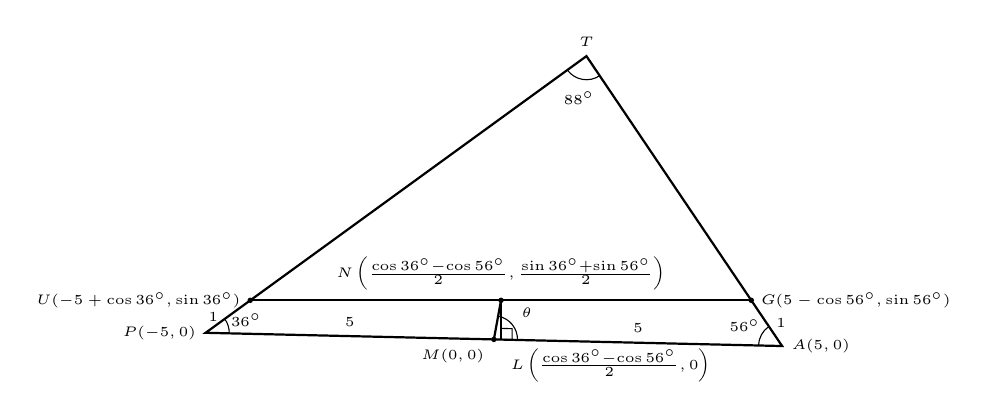
\begin{tikzpicture}[scale=0.7]
    \coordinate (A) at (11.6, 0.59);
    \coordinate (P) at (1.14, 0.83);
    \coordinate (T) at (8.05, 5.85);
    \coordinate (M) at (6.37, 0.71);
    \coordinate (N) at (6.5, 1.42);
    \coordinate (G) at (11.04, 1.42);
    \coordinate (U) at (1.95, 1.42);
    \coordinate (L) at (6.5, 0.71);

    \coordinate (V1) at (0, 0);
    \coordinate (V2) at (12, 0);
    \coordinate (V3) at (1.7, 0);
    \coordinate (V4) at (10.79, 0);
    \coordinate (V5) at (6.25, 0);

    \draw[thick] (A) -- (P) -- (T) -- cycle;
    \draw[thick] (G) -- (U);
    \draw[thick] (M) -- (N);

    \draw[thick] (N) -- (L);

    \tkzMarkRightAngle[size=.2](N,L,A);

    \foreach \n in {G, U, M, N}
        \node at (\n)[circle,fill,inner sep=0.7pt]{};
    
    \draw pic["\tiny $36^\circ$", draw=black, angle radius=0.3cm, angle eccentricity=1.8] {angle=A--P--T};
    \draw pic["\tiny $56^\circ$", draw=black, angle radius=0.3cm, angle eccentricity=1.8] {angle=T--A--P};
    \draw pic["\tiny $88^\circ$", draw=black, angle radius=0.3cm, angle eccentricity=1.8] {angle=P--T--A};
    \draw pic["\tiny $\theta$", draw=black, angle radius=0.3cm, angle eccentricity=1.8] {angle=A--M--N};
    
    \node[right] at (A) {\tiny $A (5, 0)$};
    \node[left] at (P) {\tiny $P (-5, 0)$};
    \node[above] at (T) {\tiny $T$};
    \node[left] at (U) {\tiny $U (-5 + \cos36^\circ, \sin36^\circ)$};
    \node[right] at (G) {\tiny $G (5 - \cos56^\circ, \sin56^\circ)$};
    \node[above] at (N) {\tiny $N \left( \frac{\cos36^\circ - \cos56^\circ}{2}, \frac{\sin36^\circ + \sin56^\circ}{2} \right)$};
    \node[below left] at (M) {\tiny $M(0,0)$};
    \node[below right] at (L) {\tiny $L \left( \frac{\cos36^\circ - \cos56^\circ}{2}, 0 \right)$};
    \node[above] at ($(P)!0.5!(M)$) {\tiny $5$};
    \node[above] at ($(M)!0.5!(A)$) {\tiny $5$};
    \node[left] at ($(P)!0.5!(U)$) {\tiny $1$};
    \node[right] at ($(G)!0.5!(A)$) {\tiny $1$};
\end{tikzpicture}
\end{center}
Consider the right triangle $NML$. It is evident that $\tan\theta = \frac{\frac{\sin36^\circ + \sin56^\circ}{2}}{\frac{\cos36^\circ - \cos56^\circ}{2}}$.
\begin{align*}
    \tan\theta
    &= \frac{\sin36^\circ + \sin56^\circ}{\cos36^\circ - \cos56^\circ} \\[0.5em]
    &= \frac{2 \sin46^\circ \cos10^\circ}{2 \sin46^\circ \sin10^\circ} \\[0.5em]
    &= \frac{\sin80^\circ}{\cos80^\circ} \\[0.5em]
    &= \tan80^\circ
\end{align*}
Because $\theta$ is an acute angle, the measure of the angle must be $\boxed{\textbf{(E) } 80}$.


\end{document}
